\documentclass[dvipdfmx]{jarticle}
\pagestyle{empty}
\usepackage{tikz}
\usetikzlibrary{shapes,calc}
\begin{document}
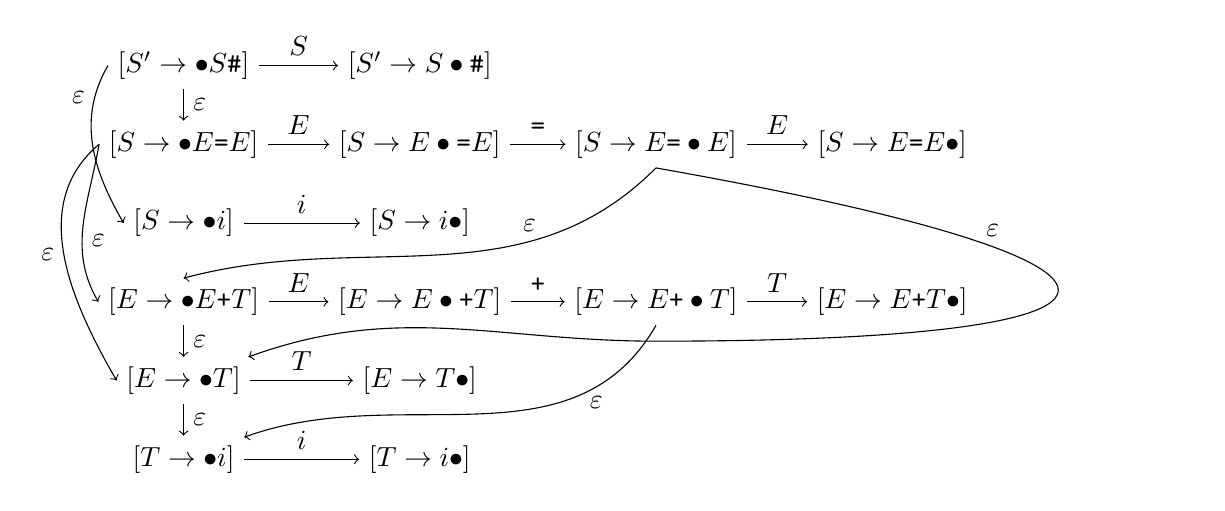
\begin{tikzpicture}
  \node (N0) at (0,0) {$[S'\rightarrow\bullet S\texttt{\#}]$};
  \node (N1) at ($(N0)+(3,0)$) {$[S'\rightarrow S\bullet\texttt{\#}]$};
  \node (N2) at ($(N0)+(0,-1)$) {$[S\rightarrow\bullet E\texttt{=}E]$};
  \node (N3) at ($(N2)+(3,0)$) {$[S\rightarrow E\bullet\texttt{=}E]$};
  \node (N4) at ($(N3)+(3,0)$) {$[S\rightarrow E\texttt{=}\bullet E]$};
  \node (N5) at ($(N4)+(3,0)$) {$[S\rightarrow E\texttt{=}E\bullet]$};
  \node (N6) at ($(N2)+(0,-1)$) {$[S\rightarrow\bullet i]$};
  \node (N7) at ($(N6)+(3,0)$) {$[S\rightarrow i\bullet]$};
  \node (N8) at ($(N6)+(0,-1)$) {$[E\rightarrow\bullet E\texttt{+}T]$};
  \node (N9) at ($(N8)+(3,0)$) {$[E\rightarrow E\bullet\texttt{+}T]$};
  \node (N10) at ($(N9)+(3,0)$) {$[E\rightarrow E\texttt{+}\bullet T]$};
  \node (N11) at ($(N10)+(3,0)$) {$[E\rightarrow E\texttt{+}T\bullet]$};
  \node (N12) at ($(N8)+(0,-1)$) {$[E\rightarrow\bullet T]$};
  \node (N13) at ($(N12)+(3,0)$) {$[E\rightarrow T\bullet]$};
  \node (N14) at ($(N12)+(0,-1)$) {$[T\rightarrow\bullet i]$};
  \node (N15) at ($(N14)+(3,0)$) {$[T\rightarrow i\bullet]$};

  \path[->] (N0) edge [above] node {$S$} (N1);
  \path[->] (N0) edge [right] node {$\varepsilon$} (N2);
  \path[->] (N2) edge [above] node {$E$} (N3) (N3) edge [above] node {$\texttt{=}$} (N4)
            (N4) edge [above] node {$E$} (N5);
  \path[->] (N6) edge [above] node {$i$} (N7);
  \path[->] (N0.west) [out=240,in=120] edge [left,pos=0.2] node {$\varepsilon$} (N6.west);
  \path[->] (N2.west) [out=260,in=120] edge [right,pos=0.6] node {$\varepsilon$} (N8.west);
  \path[->] (N2.west) [out=220,in=120] edge [left] node {$\varepsilon$} (N12.west);
  \path[->] (N4.south) [out=225,in=15] edge [above,pos=0.3] node {$\varepsilon$} (N8.north);
  \path[-] (N4.south) [out=350,in=0,looseness=8] edge [above,pos=0.3] node {$\varepsilon$} ($(N12)+(6,0.5)$);
  \path[->] ($(N12)+(6,0.5)$) [out=180,in=20] edge (N12);
  \path[->] (N8) edge [right] node {$\varepsilon$} (N12);
  \path[->] (N8) edge [above] node {$E$} (N9);
  \path[->] (N9) edge [above] node {$\texttt{+}$} (N10);
  \path[->] (N10) edge [above] node {$T$} (N11);
  \path[->] (N12) edge [above] node {$T$} (N13);
  \path[->] (N12) edge [right] node {$\varepsilon$} (N14);
  \path[->] (N14) edge [above] node {$i$} (N15);
  \path[->] (N10.south) [out=240,in=20] edge [below,pos=0.2] node {$\varepsilon$} (N14);
\end{tikzpicture}
\end{document}